\documentclass[a4paper,14pt]{article}

\usepackage{comment} % Para comentar várias linhas ao mesmo tempo

%matemática
\usepackage{amsmath}
\usepackage{amssymb}

%diagramação
\usepackage{extsizes}
\everymath{\displaystyle}
\usepackage{geometry}
\usepackage{fancyhdr}
\usepackage{multicol}
\usepackage{graphicx}
\usepackage[brazil]{babel}
\usepackage[shortlabels]{enumitem}
\usepackage{cancel}
\usepackage{textcomp}
\usepackage{tcolorbox}

%tabelas
\usepackage{array} % Para melhor formatação de tabelas
\usepackage{longtable}
\usepackage{booktabs}  % Para linhas horizontais mais bonitas
\usepackage{float}   % Para usar o modificador [H]
\usepackage{caption} % Para usar legendas em tabelas
\usepackage{wrapfig} % Para usar tabelas e figuras flutuantes

\begin{comment}
%tikzpicture
\usepackage{tikz}
\usepackage{scalerel}
\usepackage{pict2e}
\usepackage{tkz-euclide}
\usetikzlibrary{calc}
\usetikzlibrary{patterns,arrows.meta}
\usetikzlibrary{shadows}
\usetikzlibrary{external}
\end{comment}
	
%pgfplots
\usepackage{pgfplots}
\pgfplotsset{compat=newest}
\usepgfplotslibrary{statistics}
\usepgfplotslibrary{fillbetween}

%colours
\usepackage{xcolor}



\columnsep=2cm
\hoffset=0cm
\textwidth=8cm
\setlength{\columnseprule}{.1pt}
\setlength{\columnsep}{2cm}
\renewcommand{\headrulewidth}{0pt}
\geometry{top=1in, bottom=1in, left=0.7in, right=0.5in}

\pagestyle{fancy}
\fancyhf{}
\fancyfoot[C]{\thepage}

\begin{document}
	
	\noindent\textbf{6FMA76 - Matemática} 
	
	\begin{center}Divisão de decimais (I) (Versão estudante)
	\end{center}
	
	\noindent\textbf{Nome:} \underline{\hspace{10cm}}
	\noindent\textbf{Data:} \underline{\hspace{4cm}}
	
	%\section*{Questões de Matemática}
	
	\begin{multicols}{2}
		\noindent Quando o quociente de dois números inteiros não é um número inteiro, por exemplo, 1 : 4, procedemos da seguinte maneira: \\
		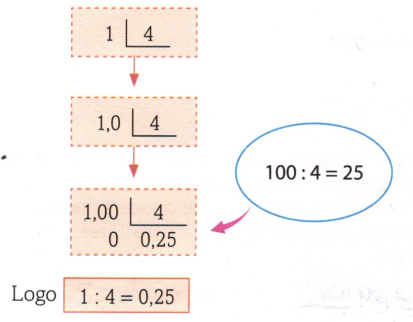
\includegraphics[width=1\linewidth]{6FMA76_imagens/imagem1}
		Para transformarmos uma fração qualquer em um número decimal, dividimos o numerador pelo denominador. \\
		Exemplo: \\
		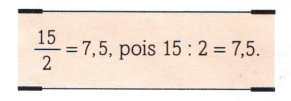
\includegraphics[width=1\linewidth]{6FMA76_imagens/imagem2}
		
		\noindent\textsubscript{-----------------------------------------------------------------------}
    	\begin{enumerate}
   			\item Determine o quociente de:
   			\begin{enumerate}[a)]
   				\item 6 por 12. \\\\\\\\
   				\item 27 por 6. \\\\\\\\
   				\item 256 por 80. \\\\\\\\
   			\end{enumerate} 
   			\item Calcule.
   			\begin{enumerate}[a)]
   				\item 14 : 50 \\\\\\\\
   				\item 166 : 80 \\\\\\\\
   				\item 500 : 160 \\\\\\\\
   			\end{enumerate} 
   			\item Um prêmio de 3 quilogramas de ouro foi dividido igualmente entre 750 ganhadores. Quanto recebeu cada um? \\
   			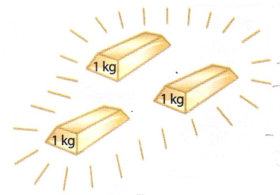
\includegraphics[width=0.5\linewidth]{6FMA76_imagens/imagem3} \newpage
   			\item Transforme as frações a seguir em numerais decimais.
   			\begin{enumerate}[a)]
   				\item $\frac{42}{10}$ \\\\\\\\\\
   				\item $\frac{4}{9}$ \\\\\\\\\\
   				\item $\frac{943}{100}$ \\\\\\\\\\
   				\item $\frac{16}{15}$ \\\\\\\\\\
   				\item $\frac{12}{9}$ \\\\\\\\\\
   			\end{enumerate}
   			\item Determine o quociente de:
   			\begin{enumerate}[a)]
   				\item 7 por 8. \\\\\\\\
   				\item 255 por 60. \\\\\\\\
   				\item 7 por 5. \\\\\\\\
   				\item 19 por 4. \\\\\\\\
   				\item 39 por 12. \\\\\\\\
   				\item 150 por 4. \\\\\\\\
   				\item 51 por 50. \\\\\\\\
   				\item 302 por 25. \\\\\\\\
   				\item 14 por 175. \newpage
   			\end{enumerate}
   			\item Transforme as frações a seguir em numerais decimais e indique quais delas são dízimas periódicas simples:
   			\begin{enumerate}[a)]
   				\item $\frac{23}{10}$ \\\\\\\\\\
   				\item $\frac{9}{4}$ \\\\\\\\\\
   				\item $\frac{924}{100}$ \\\\\\\\\\
   				\item $\frac{13}{7}$ \\\\\\\\\\
   				\item $\frac{8}{3}$ \\\\\\\\\\
   				\item $\frac{35}{14}$ \\\\\\\\\\
   				\item $\frac{4}{9}$ \\\\\\\\\\
   				\item $\frac{15}{8}$ \\\\\\\\\\
   				\item $\frac{7}{14}$ \\\\\\\\\\
   			\end{enumerate}
   			\item Antônio foi um dos ganhadores da loteria esportiva do fim de ano e recebeu R\$ 676,00, assim como os outros vencedores. Se o prêmio foi de R\$ 141.960,00, qual foi o número de ganhadores desse prêmio? \newpage
   			\item Entre os números 2, 3, 4, ..., 9, quais nunca geram dízimas periódicas quando aparecem como denominadores?
   		\end{enumerate}
        $~$ \\ $~$ \\ $~$ \\ $~$ \\ $~$ \\ $~$ \\ $~$ \\ $~$ \\ $~$ \\ $~$ \\ $~$ \\ $~$ \\ $~$ \\ $~$ \\ $~$ \\ $~$ \\ $~$ \\ $~$ \\ $~$ \\ $~$ \\ $~$ \\ $~$ \\ $~$ \\ $~$ \\ $~$ \\ $~$ \\ $~$ \\ $~$ \\ $~$ \\ $~$ \\ $~$ \\ $~$ \\ $~$ \\ $~$ \\ $~$ \\ $~$ \\ $~$ \\ $~$ \\ $~$ \\ $~$ \\ $~$ \\ $~$ \\ $~$ \\ $~$ \\ $~$ \\ $~$ \\ $~$ \\ $~$ \\ $~$ \\ $~$ \\ $~$ \\ $~$ \\ $~$ \\ $~$ \\ $~$ \\ $~$ \\ $~$ \\ $~$ \\ $~$ \\ $~$ \\ $~$ \\ $~$ \\ $~$ \\ $~$ \\ $~$ \\ $~$ \\ $~$ \\ $~$ \\ $~$ \\ $~$ \\ $~$ \\ $~$ \\ $~$ \\ $~$ \\ $~$ \\ $~$ \\ $~$ \\ $~$ 
        \end{multicols}
\end{document}